\documentclass{article}
\usepackage[margin=1.2in]{geometry}
\setlength\parindent{0pt}

%%%%%%%%%%%%%%%%%%%%%%%%%%%%%%%%%
\usepackage{enumitem}
\newlist{SubItemList}{itemize}{1}
\setlist[SubItemList]{label={$-$}}

\usepackage{algorithm,algpseudocode}
\usepackage{amsfonts}

\usepackage{graphicx}
\graphicspath{{./Figures/}}

\usepackage{hyperref}
\hypersetup{
    colorlinks=true,
    linkcolor=blue,
    filecolor=magenta,      
    urlcolor=cyan,
}

\newcommand{\mat}[1]{\mathbf{#1}} 

\newcommand{\todo}[1]{\textbf{\textcolor{red}{#1}}}

\let\OldItem\item
\newcommand{\SubItemStart}[1]{%
    \let\item\SubItemEnd
    \begin{SubItemList}[resume]%
        \OldItem #1%
}
\newcommand{\SubItemMiddle}[1]{%
   \OldItem #1%
}
\newcommand{\SubItemEnd}[1]{%
    \end{SubItemList}%
    \let\item\OldItem
    \item #1%
}
\newcommand*{\SubItem}[1]{%
    \let\SubItem\SubItemMiddle%
    \SubItemStart{#1}%
}%

%%%%%%%%%%%%%%%%%%%%%%%%%%%%%%%%%

\begin{document}

\begingroup  
  \centering
  \LARGE Large-Scale Dimensionality Reduction and Feature Learning for Protein Analysis \footnote{The full implementation of this work is available in our \href{https://bitbucket.org/mianjy/cs600.615}{repository}.} \\[1.5em]
  \large Xiaozhou Zhou, Javad Fotouhi, Poorya Mianjy, Satya Prateek \par
\endgroup


\section{Introduction}

\paragraph{Protein fold classification} A crucial step in understanding the complex mechanism of cells is to first study the function of proteins inside the cells. Protein's function is mainly explored by studying its temporal behavior, and identifying which functional phases a protein will undergo during different time intervals. The chain of Amino Acids (Polypeptides), the building blocks of proteins, often fold into functional structures and provide different protein foldings. Based on these different geometrical structures, proteins could be classified into several functional categories. To perform low cost classification, there is a certain need for automated tools using machine learning techniques. 

\paragraph{Big data and proteins} Identifying protein's folding states are very costly with biological experiments, thus it is more efficient and accurate to compute these states by collecting the entire protein information within a certain period of time. Statistical machine learning uses these information and provides means to learn multiple features from the very large scale dataset of protein recordings. The size of the protein datasets are continuously growing in order to incorporate more information for better statistical analysis.\\

The problem tackled in this project contains a large-scale recording of Amino Acid coordinates as a time-series data of protein conformations generated by molecular dynamics simulations~\cite{nutanong2013adaptive} This data set records the coordinates of all the atoms in the protein molecule at small time intervals. The number of features is in the order of $10^4 - 10^7$, the sample size is more than 10 million, and the total size of data set is over 15Tb. Due to the high dimensionality of the protein data, there is a great interest in learning more compact and informative features for the downstram task.  One could use domain knowledge to filter the number of features to the order of $10^3$.

\subsection{Problem statement}
\paragraph{Dataset} The dataset in had contains geometrical information of the Bovine Pancreatic Trypsin Inhibitor (BPTI) protein, which is comprised of 56 Amino Acids. This protein is always at one of the 5 functional states, or sometimes in transition between these states. The dataset is labeled with respect to these 5 states. \\

The dataset is comprised of 4000 snapshots of pre-defined features $\mat{D} = \left\{ \mat{D}_i : i = \{ 1, \dots, 4000\} \right\}$  acquired from molecular analysis simulations from the geometrical information of the Amino Acids within these recordings. These files are recordings of every 0.25ms over a 1s time interval. Each of these files are comprised of 1000 snapshots  $\mat{D}_i = \left\{  \mat{D}_{i_j}: j = \{ 1, \dots, 1000 \} \right\}$ which are recorded at every $0.25 \mu$s within 0.25ms intervals. Each $\mat{D}_{i_j}$ is again comprised of 4 sets of features. $\mat{D}_{i_j}.rmsd$ contains the root-meas-square distance to each of the 5 states. $\mat{D}_{i_j}.chi1$ and $\mat{D}_{i_j}.chi2$ are dihydro angles on different sides of the protein and they range in $[-180,180]$. Lastly, $\mat{D}_{i_j}.hb$ are the number of Hydrogen atoms connected to the protein, and represents the strength of the protein.


\paragraph{Task}

This work aims at reducing the dimensionality of the feature space, and performing feature learning and classification based on separate sets of features. The goal is to define the feature set which best represents the input data with respect to the labels. The results would also be compared against $\mat{D}_{i_j}.rmsd$ which is known to be highly correlated with the labels and the protein folding states.\\

In this project, we use autoencoders as our baseline for dimensionality reduction. To speed up the training of deep networks given the huge data size, we distribute the training across multiple computers. To the best of our knowledge, the majority of recent works have aimed at parallelizing deep neural networks by incorporating GPU for acceleration, however we aim at using Spark on several CPUs for scalability.

\subsection{State-of-the-art}
\paragraph{Protein classification}
Support Vector Machines (SVMs) were used as the primary classification tool for multi-class protein folding recognition~\cite{ding2001multi}. Limitations of SVMs and Semidefinite programming in terms of memory consumption and computational cost when applied to large-scale problems are extensively discussed in \cite{tsuda2005fast}. Diffusion kernels were introduced to convert the protein network to a kernel matrix with a lower complexity to provide faster.\\

\cite{tsuda2005fast} compares different classificatin techniques, from machine learning and neural networks to statistical models and decision trees. Root Mean Square Distance (RMSD) is used as the standard alignment metric  to determine the level of similarity between proteins\cite{carugo2001normalized}. \cite{cheng2006machine} uses machine learning approaches together with information retrieval techniques towards more accurate fold recognition. To this end, pairwise structural compatibility features are extracted and classification is performed with SVMs.\\

\paragraph{Parallel autoencoders}

For large-scale input data it is more efficient to split the data into chunks and train separate autoencoders. At several stages within this training there would be need for synchronization to achieve a global neural network trained on the entire training data. The general way to achieve this is to average the updates after every iteration \cite{hinton1994autoencoders}

\paragraph{Distributed neural networks} Distributed implementation of deep neural networks with asynchronous updates have been introduced in  \cite{dean2012large, chilimbi2014project}. The general model has three layers of machines. The first set, are the data serving machines which are responsible for generating (using arbitrary transformations), preparing, pre-processing, and splitting data into chunks. These machines will provide input to the model training machines which are the actual implementation of the neural network. This layer is composed of several replicas of the neural network. Each replica is fed with distinct inputs and would train a deep neural network based on the corresponding input. The model training machines are in continuous  interaction with a global parameter server which stores the weights of a global neural network. The reads and writes to the global model all take place asynchronously. The observation is that in the presence of very large-scale data, asynchronous updates may achieve better accuracy and speedup at the same time. The enhanced accuracy could be a result of adding randomness and avoiding local minimas. Furthermore, since the weight updates are summations which are associative and cummutative, therefore over asynchronous updates not much data would get lost.

\subsection{Background}
\paragraph{Dimensionality reduction}

Owing to the recent advances in digital data collection and storage technologies, datasets are becoming so large that traditional information processing methods are inadequate to perform computation on the full data. Datasets are growing both in length and width; we have more data points, in higher dimensions. The earlier is promising as it provides more information about the underlying distribution of the data, while the latter can challenge the learning process, information processing, and inference tasks, which results in the so-called "curse of dimensionality" phenomena. For this reason, many machine learning tasks involve a form of dimensionality reduction or feature extraction, aiming at transforming the data into a lower dimensional feature space, where it is easier to extract useful information from the data. The dimensionality reduction can be useful both from a computation and a statistical viewpoint: less time is required to process the data, and fewer samples are needed to guarantee the convergence of an algorithms.\\

Traditional methods of dimensionality reduction including LLE, ISOMAP, Principle Componant Analysis (PCA) and its non-linear variant so-called "kernel PCA" have been extensively studied in the literature. Stacked Denoising Auto-encoders (SDAEs) are special kind of deep neural networks that have proved to be effective in extracting abstract representations from the data \cite{vincent2010stacked}. SDAEs and kernel based approaches provide natural and intuitive means of achieving a nonlinear transformation of the data. PCA \cite{pearson1901liii} is ubiquitous in data science and machine learning. Linear PCA, downside of Kernel PCA (because of many data), and autoencoders.

\paragraph{Autoencoder and its variants} 
Autoencoders are special types of neural networks which allow dimensionality reduction of large-scale data together with unsupervised learning of features. Autoencoder maps an input using a network of neurons to a lower dimension representation. The inverse of the network weights would be then used to reproduce the input at the output layer. Through several iterations of back- and forward-propagation, the weights of the network would be updated. The middle layers of the network (network bottleneck), known as hidden layers, would be then used as the lower dimension representation of the input features~\cite{bengio2007greedy}.\\

More reliable learning as achieved through denoising autoencoders. The idea is to let the neural network to learn more robust features (to noise). Thus, random noise is added to the input and reconstruction is performed by reproducing the input from the corrupted data~\cite{vincent2008extracting}.

\paragraph{Classification} 

Several layers of denoising autoencoders could be stacked together to form a deep neural network. This is done by using the output of one hidden layer below as the input to the current layer \cite{vincent2010stacked}. \\

SVM is another common classification technique which assumes there is a hyper plane separating data points, and optimizes to locate that hyper-plane which best separates the features. SVM suffers from low speed, and will have poor performance with large-scale data.\\

K-Nearest Neighbor (KNN) algorithm is a non-parametric lazy learning technique which performs classification based on a distance function (mostly Euclidean) to a group of labeled neighbors. In the presence of large-scale data a dimensionality reduction is performed prior to classification to avoid the curse of dimensionality.

\section{Method}
\paragraph{Environment and API} 
Spark is a fast growing high level engine for fast and distributed computation for big data applications. Spark's API supports Python, Scala, and Java syntax, and allows large-scale distributed computation in memory. Due to the in-memory computation, Spark is very suitable for iterative approaches such as common machine learning tasks. 

\paragraph{Algorithm} 
We first run separate autoencoders on different views of the data $\mat{X}_{c1}, \mat{X}_{c2}, \mat{X}_{hb}$ to reduce the dimensionality and will store them in $\mat{Z}_{c1}, \mat{Z}_{c2}, \mat{Z}_{hb}$. We used 50 hidden nodes for chi1 and chi2 features. Later, the central frames were extracted from each file and were stored in $\mat{\hat{Z}}_{c1}, \mat{\hat{Z}}_{c2}, \mat{\hat{Z}}_{hb}$, respectively. For the purpose of classification, we only considered these central features since they are the most reliable frames that we can get from the data. Moreover, having fewer number of datapoints is a more challenging task, which can better show if dimensionality reduction can significantly improve the downstream task. The steps of this algorithm is described in Alg. ~\ref{alg:the_alg}.

\begin{algorithm}
\caption{Training and classification for protein folding prediction}
\textbf{Input:}\\
$L$: Number of layers\\
$D$: Bottleneck parameters\\
$l$: Frame size \\
$xl$: feature length within sub-frame\\
$\left\{ \mat{X}_{c_1}, \mat{X}_{c_2}, \mat{X}_{r}, \mat{X}_{hb} \right\} \in \mathbb{R}^{(\frac{4e+6}{l}) \times (l . xl) } $,\\
${Y} \in \mathcal{Y}^{4000}$, $\mathcal{Y} = \{1, \dots ,5 \}$\\

\textbf{Output:} \\
$ {\tilde{Y}}_{c_1}, \tilde{Y}_{c_2}, \tilde{Y}_{hb}, \tilde{Y}, \tilde{Y}_{r} \ \in \mathcal{Y}^{\frac{4e+6}{l} } $\\
\label{alg:the_alg}
\begin{algorithmic}[1]
	\State for each feature: $\{ c_1, c_2, r, hb \}$
	\begin{itemize}
		\item Run autoencoder to learn $\mat{Z}_{features} \in \mathbb{R}^{\frac{4e+6}{l} \times D}$
		\item Extract labeled data (central features) $\hat{\mat{Z}}_{features} = \mat{Z}_{features}(S,:)$
		
		 where $S = \left\{ (i-1)\frac{1000}{l} + \frac{1000}{2l} | i \in \{1, \dots, 4000\} \right\}$
		 \item Do classification on $\mat{Z}_{features}$ using $\hat{\mat{Z}}_{features}$ as training to predict $\hat{{Y}}_{features}$
		\end{itemize} 
		
		\State Concatenate all bottleneck features $\mat{Z} = \left[ \mat{Z}_{c_1}, \mat{Z}_{c_2}, \mat{Z}_{hb} \right]$
		 \State Do classification on $\mat{Z}$ using $\hat{\mat{Z}}  = \left[ \hat{\mat{Z}}_{c_1}, \hat{\mat{Z}}_{c_2}, \hat{\mat{Z}}_{hb}  \right]$ as training and predict $\hat{{Y}}$
	\State Compare the results with rmsd: $\| \hat{Y} - \hat{Y}_r \|^2$, $\| \hat{Y_{c_1}} - \hat{Y}_r \|^2$, $\| \hat{Y}_{c_2} - \hat{Y}_r \|^2$, $\| \hat{Y}_{hb} - \hat{Y}_r \|^2$
\end{algorithmic}
\end{algorithm}

\paragraph{Synchronous} For a distributed implementation, an autoencoder is initialized and broadcasted to every other node using \textit{sc.broadcast} where \textit{sc} defines the spark context. Next, the input data is split equally among the nodes (i.e. every node will have a different input). Training would be performed on each node separately, and the data would be collected to the driver node (everything fetched to a single machine) after. Later, an averaging across all the updates takes place, and the outcome of the averaged weights are broadcasted backed to every other node at the beginning of the next iteration. This process will continue until convergence. Fig.~\ref{fig:systemOutline} demonstrates the general system outline.

\begin{figure}
  \caption{System outline}
  \centering
  \includegraphics[width=\textwidth]{SystemOutline.pdf}
  \label{fig:systemOutline}
\end{figure}

%%%%%%%%%%%%%%%%%%%%%%%%%%%%%%%%%%%%

\section{Results and Evaluation}
% 0 : 2260
% 1: 1041
% 2; 478
% 3: 119
% 4: 102
% Make a table including all the numbers above from the labels and mention that it is a very biased sampling, which could naturally lead to a poor learning

\paragraph{Experiments} In order to keep the network simple, we used an autoencoder with one hidden layer, and the size of the bottleneck varies in the range of $[50,100]$. We are using sigmoid non-linearities $\sigma(z) = \frac{1}{1+e^{-z}}$. We used $\texttt{numpy.logaddexp}$ to prevent underflows in computing the sigmoid function and corresponding derivatives. To avoid overflows, we set all activations lower that $-500$ to $-500$ which is a fair approximation. The training objective is cross-entropy: $$H(y,\hat{y}) = \sum_{i=1}^d{-y_i \log{\hat{y}_i}}$$ where $y$ is the expected output and $\hat{y}$ is the output generated by network. In the case of auto-encoders, $y$ is the training points. 

\paragraph{Cluster} To perform the computation, we use the \textbf{qp-hm1} in the \textbf{damsl} cluster. This is comprised of 8 machines,  which each has the following configuration: Centos 6.4 (Dell CS24-TY, 8-core, 72GB RAM). Docker was utilized to manage the cluster of machines. Apache Spark is used for parallelization with PySpark API.

\paragraph{Optimizer} We tested our algorithm with Stochastic Gradient Descent (SGD), SGD + momentum, Adagrad and L-BFGS \cite{avriel2003nonlinear}, and no significant difference in accuracy was observed, while SGD converged faster. 

\paragraph{Pre-processing} Original data comes in 4000 separate files, each of which corresponds to a $250 \ \mu s$ time frame and contains 1000 snapshots. We first divided each file into frames of length 10, that is, each file contains 100 datapoints. Then, we further divided the dataset into 4 ``views'' based on the features we have: ``chi1'', ``chi2'', ``hbond'' and ```rmsd''. Thus, after pre-processing, we have: $$ \mat{X}_{c_1} \in \mathbb{R}^{({4e+5}) \times 420},   \mat{X}_{c_2} \in \mathbb{R}^{({4e+5}) \times 310},   \mat{X}_{hb} \in \mathbb{R}^{({4e+5}) \times 8920},   \mat{X}_{r} \in \mathbb{R}^{({4e+5}) \times 50}.$$ Characteristics of features are given in table~\ref{tab:features}.

\begin{table}
\begin{center}
\begin{tabular}{|c|c|c|c|c|c|}
\hline
 & chi1 & chi2 & hbond & rmsd \\
\hline\hline
Dimension & 42 & 31 & 892 & 5\\
\hline
Range & $[-180 , 180]$ & $[-180 , 180]$ & $\{ 0,1,2 \}$ & 5\\
\hline
\end{tabular}
\caption{Characteristics of features \label{tab:features}}
\end{center}
\end{table}
% Normalization

\paragraph{Training and testing} We applied Multinomial Bayes, Random Forests, and K-Nearest Neighbors to evaluate the quality of each of the learned features separately, and concatenated them together. A 5-fold cross validation was used on the most “reliable” data points: the central $4000$ frames and we reported the mean accuracy together with error bars.

\paragraph{Results of serial} The entire dataset with the frame size of 10 was trained and evaluated with different classifier. The results of classification with different approaches is shown in Table~\ref{tab:rawClassifier}. The classification outcome after encoding with autoencoders are shown in Table~\ref{tab:encodedClassifier}. Table~\ref{tab:rawVSencoded} shows the comparison of raw and encoded values. The results suggest that the accuracy almost remained intact while the dimensionality was significantly reduced. \\

\begin{table}
\begin{center}
\begin{tabular}{|c|c|c|c|c|c|c|}
\hline
 $(\%)$ &\textbf{chi1} & \textbf{chi2} & \textbf{rmsd} & \textbf{Hbond}& \textbf{chi1,chi2} & \textbf{chi1,chi2,rmsd} \\
\hline\hline
\textbf{Multinomial NB} & $52 \pm 5 $  & $54 \pm 9$ & $57 \pm 0$ & $51 \pm 3 $ & $51 \pm 10 $ & $47 \pm 3$\\
\hline
\textbf{K-NN} & $47 \pm 2 $ & $48 \pm 3 $ & $46 \pm 6 $ & $48 \pm 3$ & $50 \pm 3 $ & $51 \pm 3 $\\
\hline
\textbf{Random Forests} & $57 \pm 2$ & $57 \pm 0 $ & $55 \pm 3$ & $ 57 \pm 0 $ & $57 \pm 0$ & $57 \pm 0 -09$\\
\hline
\end{tabular}
\caption{Classification comparison over raw data. The raw input files are tested with "Multinomial Naive Base", "K-Nearest Neighbours", and "Random Forests" classifiers. The classification outcome is compared against the labeled data and presented in the form of accuracy and the standard deviation in precentage. \label{tab:rawClassifier}}
\end{center}
\end{table}

\begin{table}
\begin{center}
\begin{tabular}{|c|c|c|c|c|c|}
\hline
 $(\%)$ &\textbf{chi1} & \textbf{chi2} & \textbf{chi1,chi2} \\
\hline\hline
\textbf{Multinomial NB} & $56 \pm 0$  & $56 \pm 0 $ & $56 \pm 0$ \\
\hline
\textbf{K-NN} & $45 \pm 3 $ & $50 \pm 3 $ & $50 \pm 2 $ \\
\hline
\textbf{Random Forests} & $56 \pm 0 $ & $56 \pm 3 $ & $57 \pm 0$ \\
\hline
\end{tabular}
\caption{Classification comparison over encoded data. The dimensionality of the dataset is first reduced, and then "Multinomial Naive Base", "K-Nearest Neighbours", and "Random Forests" classifiers are used on the encoded features. The results are compared with the labeled ground-truth and presented in terms of accuracy and standard deviation \label{tab:encodedClassifier}}
\end{center}
\end{table}

\begin{table}
\begin{center}
\begin{tabular}{|c|c|c|c|c|c|}
\hline
 $(\%)$ &\textbf{8-NN} & \textbf{Naive Bayse} & \textbf{Random Forest} \\
\hline\hline
\textbf{Raw data} & $55 \pm 5 $  & $57 \pm 2 $ & $57 \pm 0$ \\
\hline
\textbf{Encoded data} & $53 \pm 3 $ & $56 \pm 0 $ & $56 \pm 0$ \\
\hline
\end{tabular}
\caption{ Comparison of classification of concatinated raw and learned features \label{tab:rawVSencoded}}
\end{center}
\end{table}

The accuracy results of chi1 and chi2 features for raw and encoded data against different classifiers are illustrated in Fig.~\ref{fig:chi1_cv} and ~\ref{fig:chi2_cv}, respectively. Results show improvement with Moltinomial BN classifier for the encoded data. The classification results for raw rmsd values are shown in Fig.~\ref{fig:rmsd_raw_cv}. In this case, Multinomial NB outperformed the other two classification methods. Fig,~\ref{fig:hbonds_raw} demonstrates the classification comparison for raw Hbond features. Random Forests achieved $57 \%$ accuracy with very small variations on the Hbond features. The combination of Chi1 and Chi2 features are shown in Fig.~\ref{fig:chi1_chi2_cv}. Lastly, the combination of the three features Chi1, Chi2, and rmsd are shown in Fig.~\ref{fig:chi1_chi2_r}.

\begin{figure}
  \caption{Chi1 classifier performance for raw and encoded data}
  \centering
  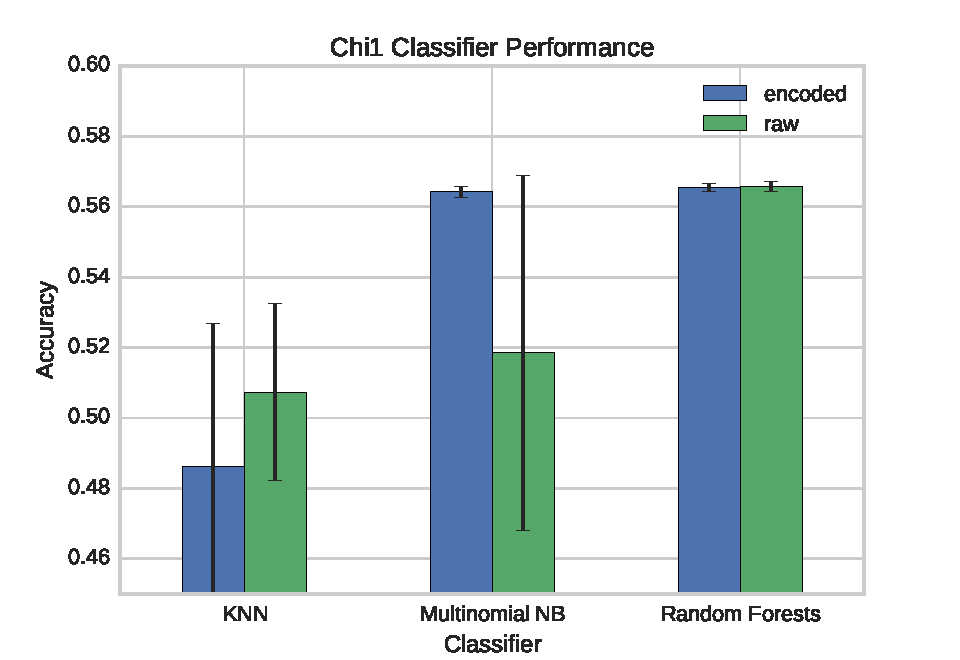
\includegraphics[width=0.8\textwidth]{chi1_cv.pdf}
  \label{fig:chi1_cv}
\end{figure}

\begin{figure}
  \caption{Chi2 classifier performance for raw and encoded data}
  \centering
  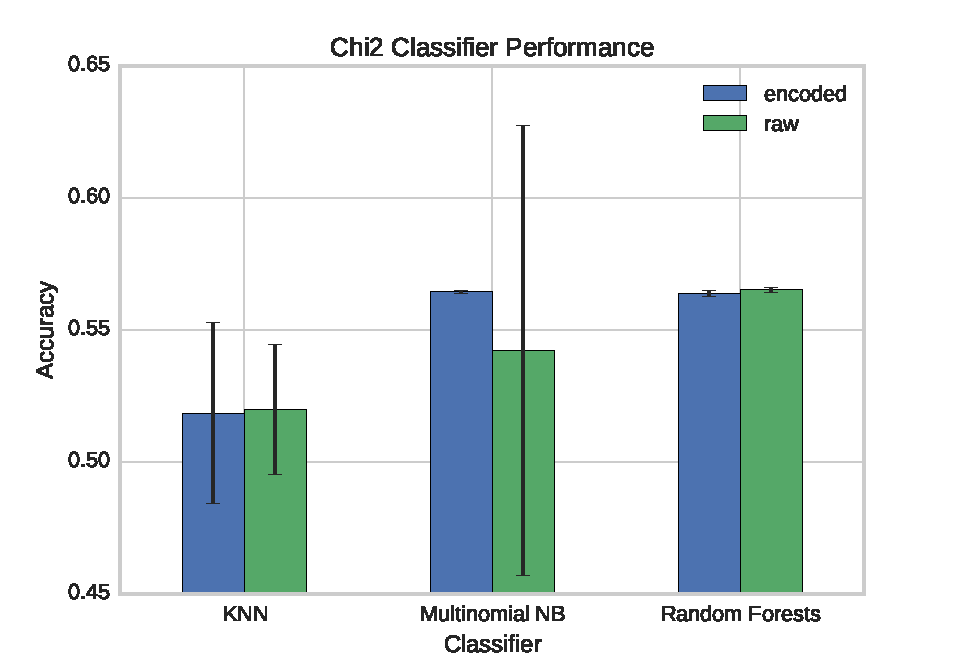
\includegraphics[width=0.8\textwidth]{chi2_cv.pdf}
  \label{fig:chi2_cv}
\end{figure}

\begin{figure}
  \caption{RMSD classifier performance for raw data}
  \centering
  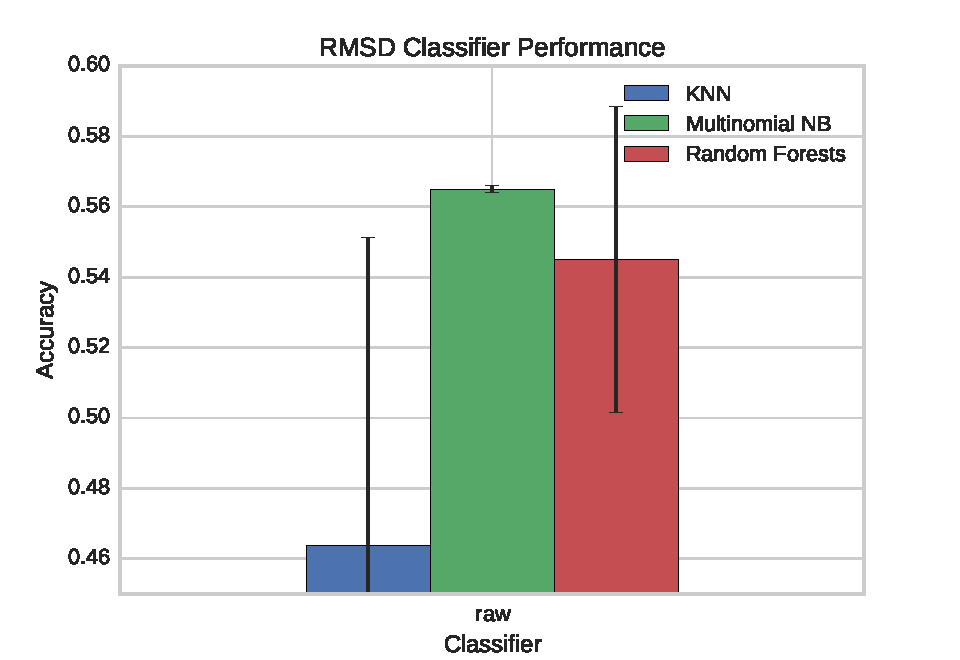
\includegraphics[width=0.8\textwidth]{rmsd_raw_cv.pdf}
  \label{fig:rmsd_raw_cv}
\end{figure}

\begin{figure}
  \caption{Hbond classifier performance for raw data}
  \centering
  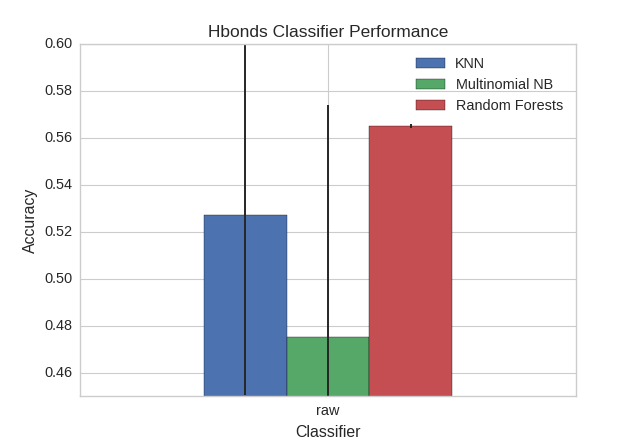
\includegraphics[width=0.8\textwidth]{hbonds_raw.png}
  \label{fig:hbonds_raw}
\end{figure}

\begin{figure}
  \caption{Combined Chi1 and Chi2 classifier performance for raw and encoded data}
  \centering
  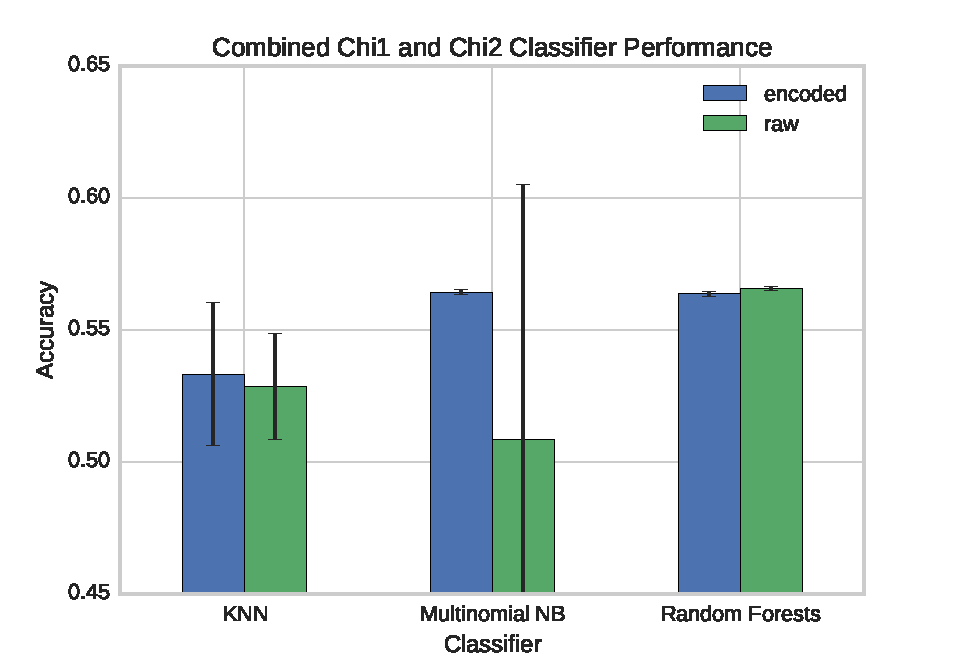
\includegraphics[width=0.8\textwidth]{chi1_chi2_cv.pdf}
  \label{fig:chi1_chi2_cv}
\end{figure}

\begin{figure}
  \caption{Combined Chi1, Chi2, and RMSD classifier performance for raw data}
  \centering
  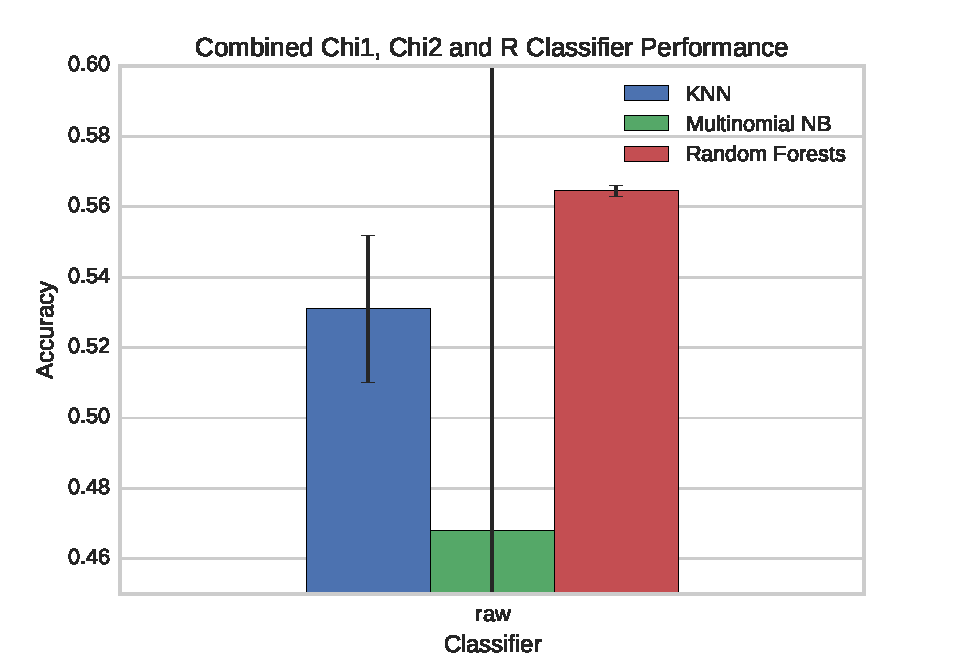
\includegraphics[width=0.8\textwidth]{chi1_chi2_r.pdf}
  \label{fig:chi1_chi2_r}
\end{figure}

\paragraph{Results of parallel synchronization} The parallel implementation of the autoencoder is tested against different number of nodes ranging from 1 to 64. The speedup plot for a subset of input files is shown in Fig.~\ref{fig:spark_speedup}, which results in nearly linear speedup up to 16 nodes. 

\begin{figure}
  \caption{Speedup plot from 1 to 64 threads}
  \centering
  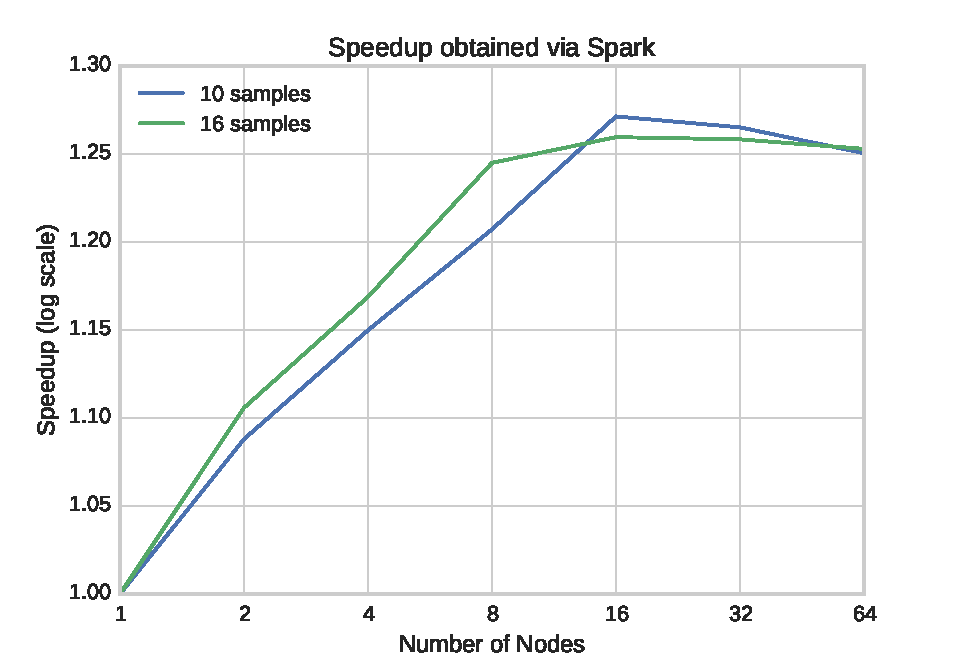
\includegraphics[width=0.8\textwidth]{spark_speedup.pdf}
  \label{fig:spark_speedup}
\end{figure}

\paragraph{Error measures to the labels} The classification accuracy is measured by comparing the results directly with pre-defined labels. To this end, we use 0-1 loss functions and will compute the percentage of matching among classes.

%%%%%%%%%%%%%%%%%%%%%%%%%%%%%%%%%%%%%%

\section{Discussion and Conclusion}
\paragraph{Summary} In this project, we considered the problem of non-linear dimensionality reduction of protein data. We used vanilla SGD together with decaying rate $\frac{1}{\sqrt{n}}$to train an autoencoder with sigmoid activation functions, where the objective is cross-entropy with $\ell_1$ penalty. We then used several classification methods to evaluate the quality of the learned features. Experimental results suggest a 98.5 $(\%)$ decrease in the dimensionality while preserving the classification accuracy. Once we have this results in a serial setting, we used Spark to parallelize the training on autoencoders in a synchronous manner, where we observed $\times$3.15 speedup using 16 nodes.

\paragraph{Conclusion} With a high-dimensional setting, where the dimension of the input is in the order of the number of data points, dimensionality reduction and feature learning would become an essential task for downstream tasks such as classification or any kind of inference. In this problem, the dimensionality of input $d=(42+31+892)*10 \approx 10k$ is relatively big compared to the number of "reliable" samples $\sim 4k - 40k$ available. Since the structure of the data is (supposedly) highly non-linear, linear dimensionality reduction methods (e.g. PCA) may not be the right choice. Here, we incorporate autoencoders, which are reportedly shown to be very useful for leaning non-linear structures in  data so-called "manifold learning". In our case, we showed that using an autoencoder can decrease the dimensionality of data from $\sim 10k$ to $150$, while preserving the downstream classification accuracy.\\

Due to time constraints, we are skipping vital hyper-parameter tuning in this project, which have certainly affected our results. To illustrate, the frame length $\ell$, number of hidden units, number of neighbors $k$ in KNN, regularization parameter in the objective, and the initial learning rate $\eta_0$ for SGD training which should be tuned in a typical cross-validation framework. However, we still achieve reasonable results compared to the raw data without any further tuning.\\

As shown in the results, the combination of Chi1 and Chi2 features together outperforms the combination of Chi1, Chi2, and Hbond all together. The decrease in accuracy could be the natural cause of applying autoencoders to the categorical data (Hbond).

\paragraph{Future direction} This aforementioned implementation could be further improved by using "wiser" methods to fuse different views. Currently, the learned features are simply concatenated from separate autoencoders, which is arguably \underline{not} the best way. The more interesting approach could be performing multi-view learning methods such as CCA~\cite{hotelling1936relations} to "learn" a fusion instead of naive concatenation.\\

A different approach would be using neural network models which are more suited for classifying functional data. Considering the fact that protein data is a time series information, one could use networks such as RNN~\cite{lang1990time} or LSTM~\cite{hochreiter1997long} which have shown promising results on modeling time sequences in core AI tasks, namely speech~\cite{graves2013speech} and NLP~\cite{mikolov2010recurrent}.\\

To benefit more from the power of autoencoders, one should consider training a network with larger number of hidden layers. The idea of SDAE has been studied in the literature and showed to be useful in producing "deeper" representations.\\

To better optimize the algorithm one could also use Spark's machine learning library (MLlib), or Apache Ignite to leverage shared memory computation to achieve fast asynchronous updates. Though we did not test the asynchronous updates, but our expectation is that its speedup should not be significant. This is mainly because with small number of iterations and few machines, the number of synchronizations are very few, thus not much time is spent for nodes waiting on the others to finish computation. On the scale of this computation, few machines ($<10$) seems fairly enough.

\bibliographystyle{ieeetr}
\bibliography{references}

\end{document}